% !TeX root = ../tesis.tex

%-----------------------------------------------------------------------
\section{Justificación}
\label{sec:justificacion}
%-----------------------------------------------------------------------

La pertinencia de esta investigación se sustenta en dar una alternativa y
explicación a la fragmentación
estructural de la movilidad en la Zona Metropolitana del Valle de México, la
cual se manifiesta de forma
diferenciada según el modelo de \textbf{Contornos Metropolitanos} definido en
los diagnósticos técnicos de movilidad urbana.

En la \textbf{Ciudad Central} y el \textbf{Primer Contorno}, el sistema presenta
una alta densidad de infraestructura
de transporte masivo que, si bien garantiza una cobertura amplia, genera una
centralización excesiva de los flujos.
Esta configuración radial-concéntrica obliga a que la mayoría de los viajes
metropolitanos atraviesen nodos
críticos como Pantitlán, Indios Verdes o Taxqueña, saturando su capacidad
operativa y elevando la vulnerabilidad
del sistema ante cualquier falla en estos puntos neurálgicos.

Por el contrario, el \textbf{Tercer Contorno} (o \textit{Middle-Ring}), que
alberga zonas de alta demanda y
servicios críticos como la Zona de Hospitales y Ciudad Universitaria, carece de
una conectividad transversal robusta.
La ausencia de rutas perimetrales eficientes en esta franja obliga a los
usuarios a realizar trayectos multimodales hacia el núcleo central
para luego retornar a zonas periféricas aledañas, lo que se traduce
matemáticamente en un incremento del Índice de Ruta Directa ($DI$)
y una pérdida de eficiencia geométrica.

Finalmente, el análisis se extiende al \textbf{Cuarto Contorno} (periferia
profunda), donde se registran los tiempos de traslado más elevados del sistema,
superando en promedio los 122 minutos por viaje. En este sector, la dependencia
del transporte de baja capacidad y la fragmentación de los servicios
alimentadores
hacia la red masiva profundizan la desigualdad socioespacial
\citep{semovi2020diagnostico}.
Esta configuración justifica la exploración de alternativas perimetrales
que descompriman los nodos del núcleo central y reduzcan los tiempos de
traslado en los contornos más alejados.


\begin{quote}
``Otro nivel de complejidad se debe a que los servicios que conforman el sistema
de
movilidad no fueron diseñados de origen para integrar una red física de
transporte
para la Ciudad de México, ni menos aún, para dar servicio a la Zona
Metropolitana
del Valle de México. Por lo anterior, su integración es uno de los puntos
prioritarios
a atender con el fin de garantizar un servicio de movilidad integrado, digno e
incluyente.'' \citep[p.~XX]{semovi2020diagnostico}
\end{quote}


\begin{figure}[htbp]
    \centering
    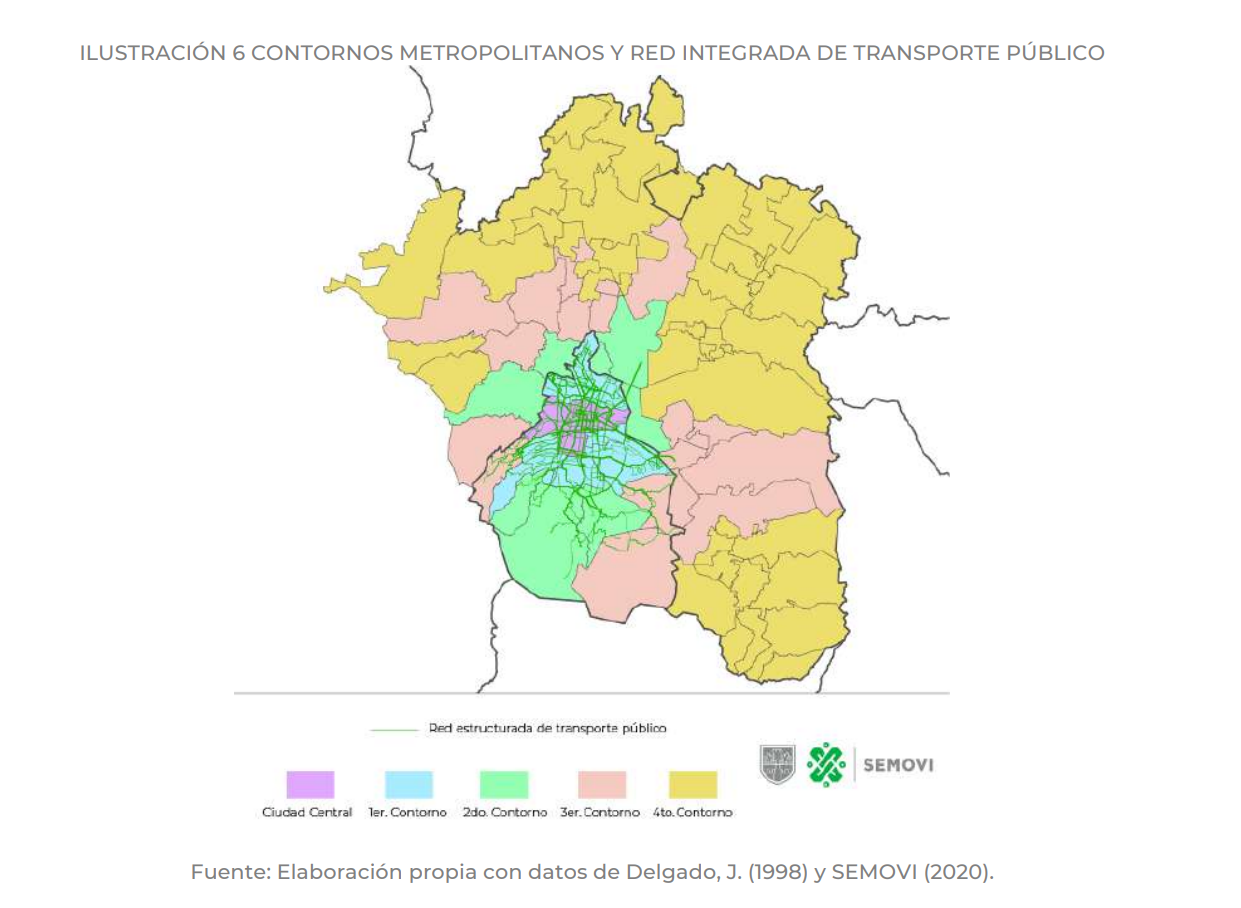
\includegraphics[width=0.80\textwidth]{Figures/Cap1/SEMOVITC}
    \caption[Contornos Metropolitanos]{Contornos Metropolitanos y red de transporte
    público integrada.}
    \label{fig:semovi-contornos}
\small
\textit{Fuente: Diagnóstico Técnico de Movilidad para el Programa Integral de
    Movilidad (2019--2024, p.~16).}
\end{figure}

Esta falta de integración se refleja en la calidad de los viajes y genera
severos
problemas de desigualdad en el acceso a la capital. Conforme aumenta la
distancia
entre la red de transporte masivo y las zonas habitacionales, más viajes
multimodales
se tienen que realizar, lo que implica más tiempo y gastos de traslado
\citep{semovi2020diagnostico}.

El diagnóstico de SEMOVITC evidencia que las demarcaciones ubicadas en el
\textbf{Tercer Contorno},
con especial énfasis en las alcaldías del sur de la metrópoli, enfrentan un
déficit estructural de
accesibilidad derivado de la configuración radial-concéntrica de la red masiva.
Dicha desconexión topográfica justifica la necesidad técnica de explorar
alternativas perimetrales
que articulen transversalmente estas zonas sin la obligatoriedad de converger en
el núcleo central,
reduciendo así la centralidad de intermediación de los nodos históricos.

Actualmente, la carencia de infraestructura de alta capacidad en estos sectores
delega la movilidad
en el transporte público concesionado ---compuesto primordialmente por
colectivos, autobuses y vagonetas---,
el cual es utilizado por el 48\% de la población en al menos uno de sus tramos
de viaje \citep{semovi2020diagnostico}.
Este servicio opera mayoritariamente bajo el esquema ``hombre-camión'', lo que
fomenta una competencia ineficiente por
el pasaje y eleva los costos asociados a la seguridad vial.
En el marco del análisis topológico propuesto, esta dependencia de un servicio
poco confiable y fragmentado constituye la principal fuente de
\textit{vulnerabilidad funcional} en la periferia, lo que justifica la
evaluación de alternativas anillares como mecanismo de recalibración
geométrica de la red.

Un elemento significativo es el uso de un medio de transporte que presente una
geometría diferente a la convencional. Las llamadas rutas radiales son el tipo
más
común:

\begin{quote}
``[\ldots] En ciudades mayores a los 300,000 habitantes este tipo de rutas
empieza
a ser ineficiente ya que concentra los movimientos y no considera las
necesidades
que se presentan entre otras áreas urbanas. Esto induce a que la distribución
del
servicio se encuentre limitada a ciertas áreas de la ciudad y concentre las
terminales
en las zonas de mayor densidad.'' \citep[p.~XX]{molinero2002}
\end{quote}

\begin{figure}[htbp]
    \centering
    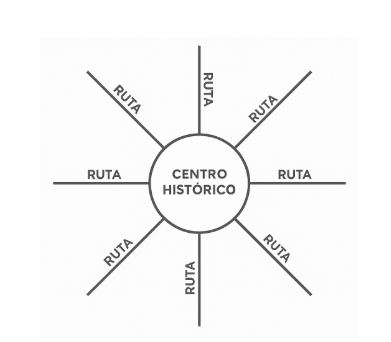
\includegraphics[width=0.55\textwidth]{Figures/Cap1/ETR}
    \caption[Esquema de transporte radial]{Esquema del sistema de transporte radial.}
    \label{fig:transporte-radial}
    \small\textit{Fuente: Elaboración propia.}
\end{figure}

En cambio, las rutas circulares sirven de rutas conectoras con las radiales,
permitiendo una mejor distribución de los usuarios y una mejor utilización del
parque
vehicular. Casos típicos de este tipo son las líneas circulares de los metros de
Londres y Moscú, o los circuitos de los autobuses de Guadalajara y otras
ciudades
mexicanas \citep{molinero2002}.

\begin{figure}[htbp]
    \centering
    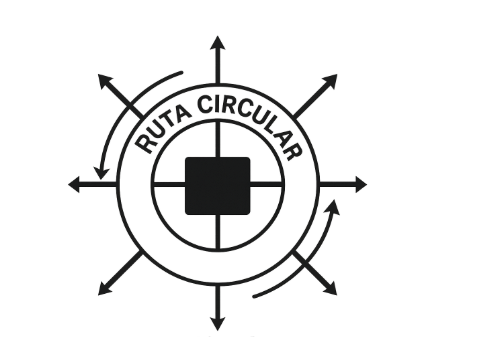
\includegraphics[width=0.55\textwidth]{Figures/Cap1/ETC}
    \caption[Esquema de transporte circular]{Esquema del sistema de transporte
    circular.}
    \label{fig:transporte-circular}
\small\textit{Fuente: Elaboración propia con base en \citet{molinero2002}.}
\end{figure}

A la fecha de realización de este estudio (2025), no existe en la Ciudad de
México alguna ruta circular que sirva de soporte para el transporte público
masivo colectivo. A pesar de que la Ciudad cuenta con una vialidad de trazo
circular ---el Anillo Periférico---, esta se ha orientado históricamente al
automóvil privado como resultado de políticas de automovilidad hegemónicas.
En este contexto, la presente investigación se justifica tanto en la necesidad
técnica de evaluar escenarios anillares hipotéticos como en el desarrollo de
una metodología replicable que facilite este tipo de análisis a planificadores
urbanos en cualquier ciudad con datos \gtfs{} disponibles.

\subsection{Tercer y Cuarto Contorno: caso de aplicación de la metodología anillar} \label{subsec:beneficiarios-contornos}
La implementación de un corredor de transporte masivo en el Anillo Periférico
tiene como objetivo principal mitigar las
desigualdades estructurales de movilidad que afectan primordialmente al Tercer
Contorno (Middle-Ring) y al Cuarto Contorno
(periferia profunda) de la ZMVM. Mientras que la Ciudad Central, el Primer
Contorno y el Segundo Contorno
—que integran las alcaldías centrales— presentan la mayor densidad de
infraestructura de transporte masivo (Metro y Metrobús),
las zonas periféricas han sido históricamente desatendidas por la red
estructurada. Esta «suposición de cobertura» centralizada se
abordará con rigor matemático en el Capítulo 3: Conceptos e Indicadores, donde
métricas como el Nivel de Cobertura (C) y la Fuerza Nodal (Ci)
permitirán cuantificar el desajuste entre la oferta de transporte y la
localización de la población en la periferia.

El análisis de los cuatro cuadrantes del Anillo Periférico como escenario
hipotético responde a la necesidad de evaluar la consolidación del llamado
\textit{Middle-Ring} o «Anillo Medio».
Según el análisis estratégico del \textit{Suburban Rail Loop} de Melbourne
\citep{suburbanrailloop2021}, estos anillos se definen
como zonas de transición que albergan infraestructuras críticas como hospitales
y universidades, pero que tienden a carecer de una conectividad
lateral robusta. Para la Ciudad de México, las alcaldías del sur (
\textbf{Tlalpan, Xochimilco y Tláhuac}) conforman funcionalmente este tercer
contorno,
operando como «parches» aislados en la trama urbana que obligan a los usuarios a
realizar viajes radiales ineficientes hacia el centro para conectar
con zonas vecinas.

Por otro lado, el Cuarto Contorno se posiciona como el beneficiario indirecto
más crítico. En esta zona, los habitantes experimentan los tiempos de
traslado más elevados de la metrópoli, superando los 122 minutos por trayecto
laboral. Al no existir rutas perimetrales, los flujos provenientes de
la periferia profunda saturan los nodos centrales del sistema, elevando la
vulnerabilidad funcional de la red. La metodología desarrollada en esta
investigación toma estos contornos como
campo de demostración: evaluar si la incorporación de corredores anillares
en los cuatro cuadrantes del Anillo Periférico reduce los indicadores de
ineficiencia topológica \citep{suburbanrailloop2021} y redistribuye los flujos
actualmente concentrados en el núcleo central.

%-----------------------------------------------------------------------
\section{Hipótesis}
\label{sec:hipotesis}
%-----------------------------------------------------------------------

La red de transporte multimodal de la \zmvm{} presenta una configuración
radial-concéntrica que genera vulnerabilidades funcionales cuantificables: una
centralidad de intermediación ($B(v)$) elevada en los nodos del núcleo central,
un Índice de Ruta Directa ($DI$) alto en los contornos periféricos y tiempos de
viaje promedio ($T$) que superan los 122 minutos en el Cuarto Contorno
\citep{semovi2020diagnostico}. Se postula que la metodología desarrollada
permite cuantificar dichas vulnerabilidades y que la incorporación hipotética
de corredores anillares en los cuatro cuadrantes del Anillo Periférico
producirá una reducción medible de los indicadores $DI$, $T$ y $B(v)$,
demostrable mediante el análisis comparativo de la red actual frente a la
red ampliada con el escenario propuesto.

%-----------------------------------------------------------------------
